Construcción Tridimensional

\begin{figure}[H]
    \centering
    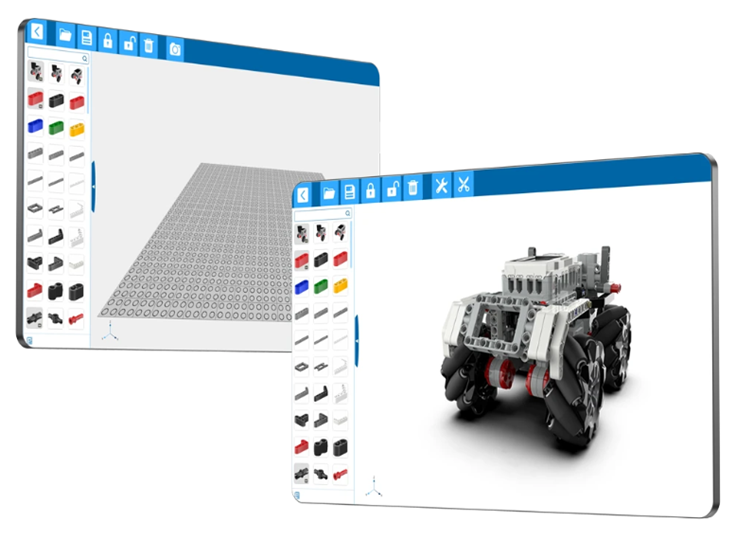
\includegraphics[scale = 0.50]{Imagenes/trid.png}
    \caption{Construcción en 3 dimensiones}{Fuente: Propia}
\end{figure}

\textbf{Columna de bloques de construcción:} Se utiliza para seleccionar los bloques de construcción necesarios. Hay 10 categorías que incluyen robots, vigas, pasadores, ejes, engranajes, componentes electrónicos, piezas decorativas, casquillos, ruedas y otros.

\textbf{Barra de búsqueda:} Puede buscar los bloques de construcción correspondientes ingresando sus nombres.

\textbf{Abrir archivo:} Abra el archivo del modelo de robot en la computadora. El formato de archivo que se puede abrir es rsr.

\textbf{Guardar archivo:} Guarde el modelo del robot en la computadora, el formato de archivo es rsr.

\textbf{Congelar bloques de construcción:} Congele los bloques de construcción seleccionados para que no participen en la coincidencia de adsorción.

Para este modo de construcción libre el software nos da una serie de herramientas como pueden ser: llantas, robots, pin, ejes, engranaje y manguito del eje ~\cite{chino}.

\begin{figure}[H]
    \centering
    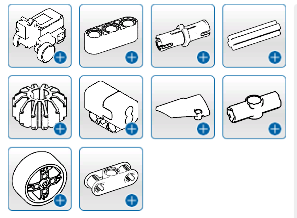
\includegraphics[scale = 0.95]{Imagenes/herramientascons.png}
    \caption{Herramientas de construcción del software}{Fuente: Propia}
\end{figure}

Esta interfaz de construcción ofrece este tipo de opciones

\begin{figure}[H]
    \centering
    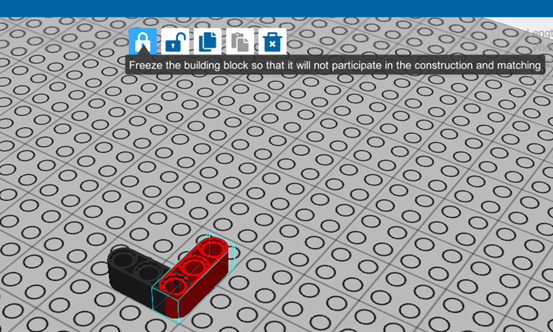
\includegraphics[scale = 0.90]{Imagenes/bloques_constr.png}
    \caption{Bloques en construcción}{Fuente: Propia}
\end{figure}

Lo que significa que se pueden congelar piezas para un mejor control a la hora de construir.
También ofrece un manual para el uso de mouse y teclado

\begin{figure}[H]
    \centering
    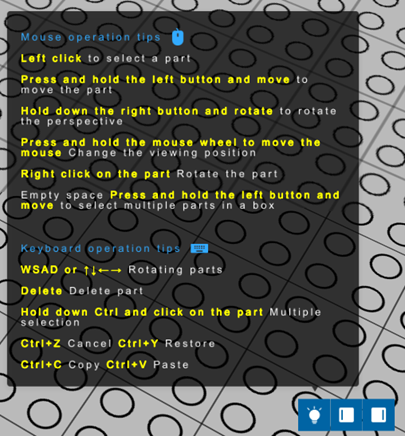
\includegraphics[scale = 0.90]{Imagenes/instruccionesRaton.png}
    \caption{Instrucciones para el uso del ratón en esta interfaz.}{Fuente: Propia}
\end{figure}

Construcción y diseño de espacios para simulación

\begin{figure}[H]
    \centering
    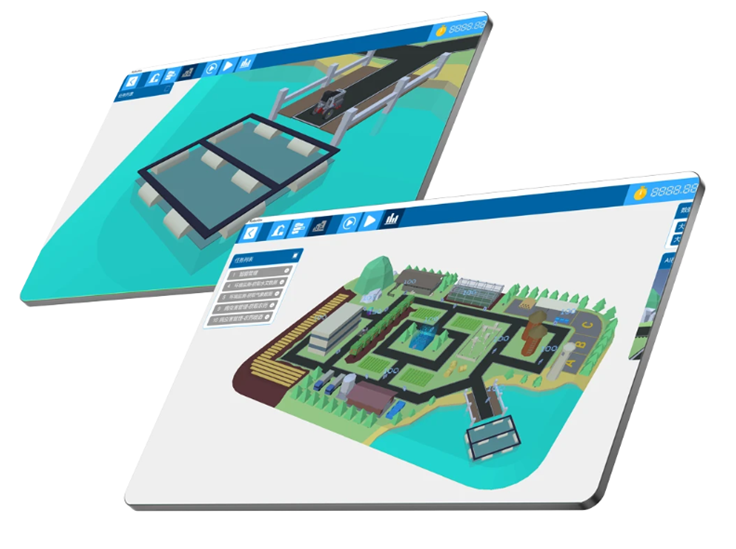
\includegraphics[scale = 0.65]{Imagenes/diseno_entorno.png}
    \caption{Interfaz de Diseño de entorno.}{Fuente: Propia}
\end{figure}

\begin{figure}[H]
    \centering
    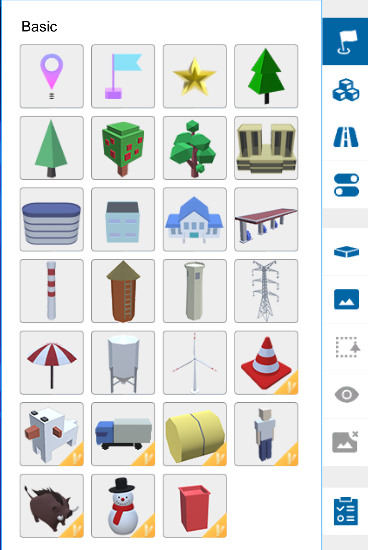
\includegraphics[scale = 0.75]{Imagenes/materiales.png}
    \caption{Materiales para diseño}{Fuente: Propia}
\end{figure}

\begin{figure}[H]
    \centering
    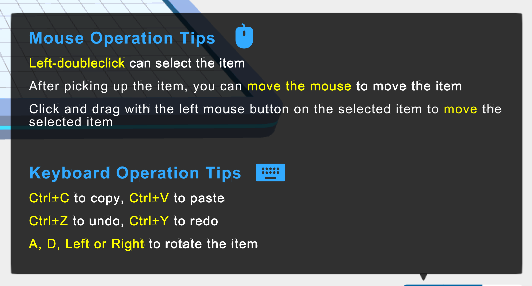
\includegraphics[scale = 0.90]{Imagenes/intr_Raton.png}
    \caption{Guía del uso del ratón}{Fuente: Propia}
\end{figure}

Simulación virtual

\begin{figure}[H]
    \centering
    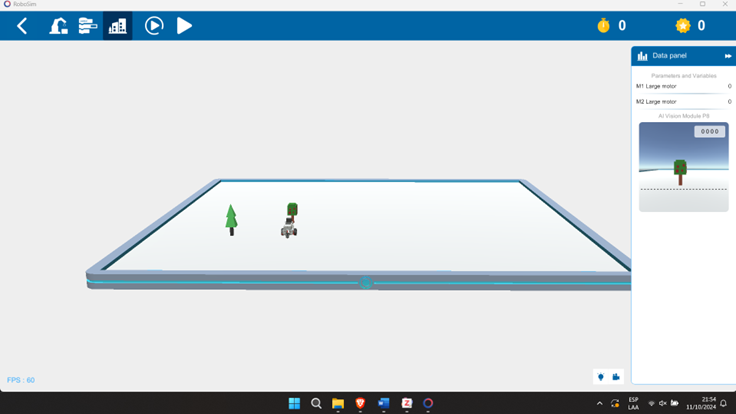
\includegraphics[scale = 0.90]{Imagenes/simulacion_virtual.png}
    \caption{Entorno de simulación virtual}{Fuente: Propia}
\end{figure}

\begin{figure}[H]
    \centering
    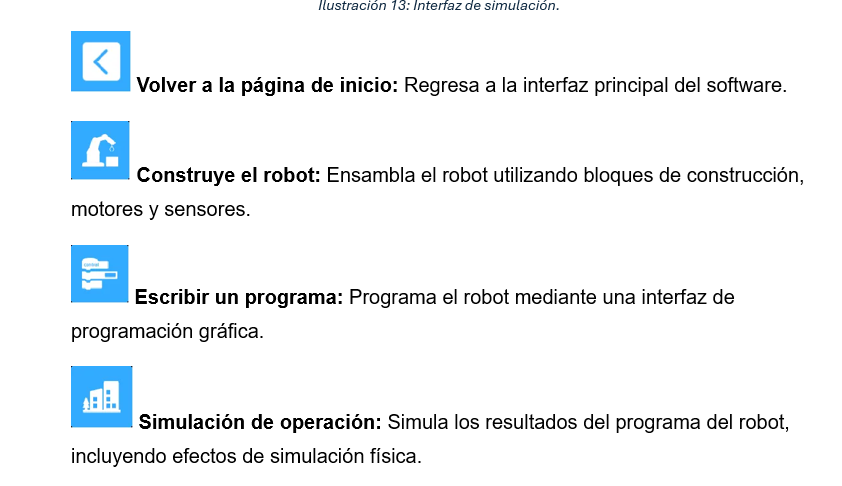
\includegraphics[scale = 0.90]{Imagenes/descripcipn_botones.png}
    \caption{Descripción de botones}{Fuente: Propia}
\end{figure}

Programación

\begin{figure}[H]
    \centering
    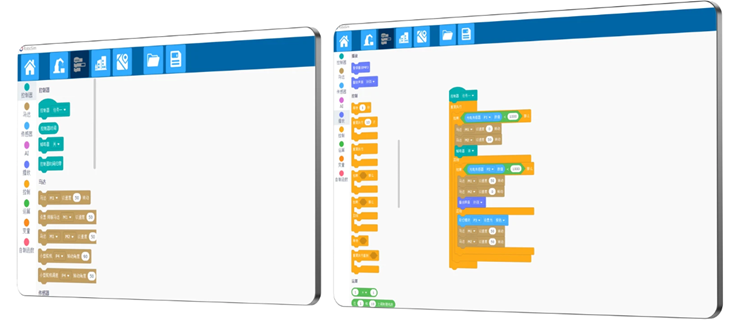
\includegraphics[scale = 0.90]{Imagenes/interfaz_prog.png}
    \caption{Interfaz de programación}{Fuente: Propia}
\end{figure}

\textbf{Tipo de columna:} Divide diferentes módulos de programación en 10 categorías.

\textbf{Módulo de programación:} El módulo de programación correspondiente que controla el robot para ejecutar diferentes instrucciones.

\textbf{Área de programación:} En esta área los módulos de programación se pueden unir para generar un programa de robot.

\textbf{Área de código:} Muestra el código de Python/C++ del programa del robot.

\begin{figure}[H]
    \centering
    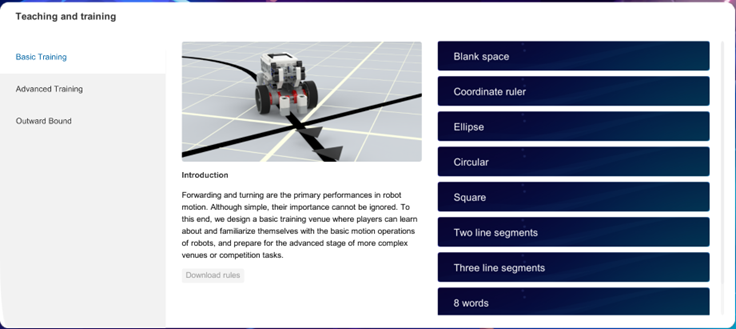
\includegraphics[scale = 0.90]{Imagenes/areas_training.png}
    \caption{Interfaz de entrenamiento}{Fuente: Propia}
\end{figure}

\begin{figure}[H]
    \centering
    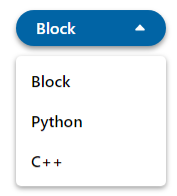
\includegraphics[scale = 0.90]{Imagenes/op_program.png}
    \caption{Tipos de programación y lenguajes}{Fuente: Propia}
\end{figure}

\textbf{Cursos}

\begin{itemize}
    \item \textbf{Curso básico:} Este curso está dirigido principalmente a estudiantes de primaria y secundaria que están expuestos a software de simulación virtual por primera vez. Los estudiantes pueden aprender el proceso de diseño, construcción y programación de robots para simulación en un mundo virtual, y gradualmente adquirir conocimientos sobre operaciones básicas, principios y aplicaciones de sensores, movimiento de robots, estructuras y algoritmos de programación, etc.
    
    \item \textbf{Curso Avanzado:} Dirigido a estudiantes que hayan completado el curso básico. A través de investigaciones entretenidas y proyectos temáticos, los estudiantes no solo consolidarán y reforzarán lo aprendido en la etapa básica, sino que también adquirirán conocimientos multidisciplinarios como movimiento físico, aplicaciones avanzadas de sensores, algoritmos complejos de programación y reconocimiento visual mediante inteligencia artificial.
     
    \item \textbf{Curso de Competencia:} Este curso está diseñado para que los participantes comprendan el proceso de competencias virtuales en línea, los requisitos de reglas, precauciones y claves para completar cada tarea en el recinto temático. Los estudiantes aprenderán habilidades de diseño y programación de robots para competencias basadas en escenarios y conocerán los métodos comunes de depuración y simulación utilizados en la competencia \cite{robosim}.
\end{itemize}

\begin{figure}[H]
    \centering
    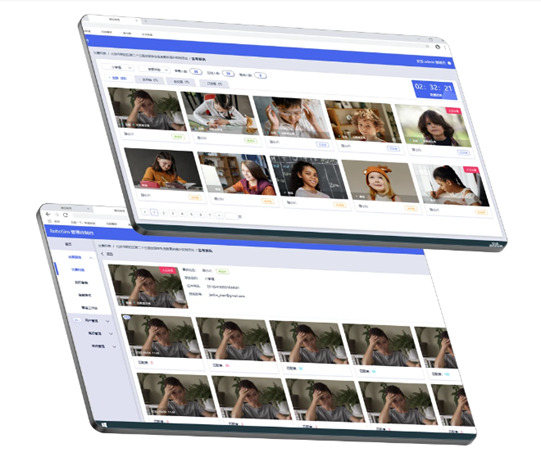
\includegraphics[scale = 0.90]{Imagenes/cursoseduc.png}
    \caption{Cursos educativos disponibles}{Fuente: Propia}
\end{figure}

\textbf{Competencia Online:} Esta plataforma ofrece competición profesional y servicios personalizados.

\begin{figure}[H]
    \centering
    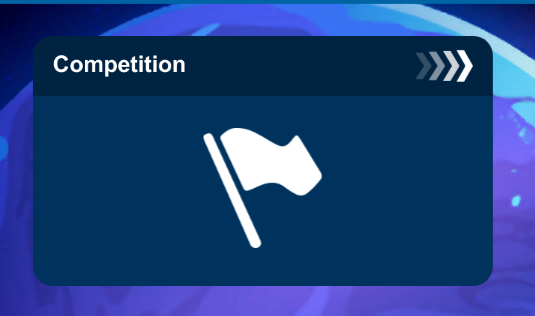
\includegraphics[scale = 0.90]{Imagenes/competir.png}
    \caption{Opción de competición}{Fuente: Propia}
\end{figure}

\begin{figure}[H]
    \centering
    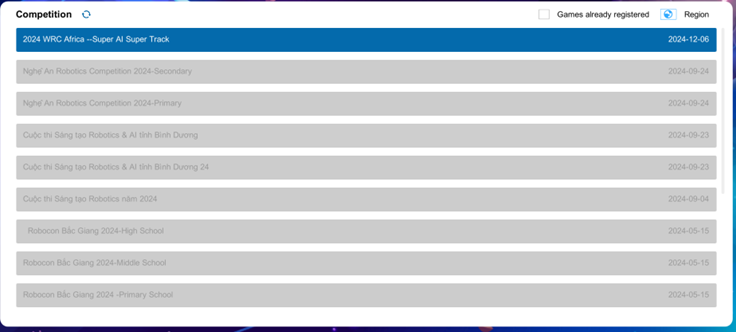
\includegraphics[scale = 0.90]{Imagenes/areas_comp.png}
    \caption{Áreas de competición}{Fuente: Propia}
\end{figure}